\subsection{DHC VISION Information Security Manager}
DHC VISION ist eine Software für Prozessmanagement, Qualität und Governance, Risk und Compliance.
Der Modulare Aufbau wird in Abbildung \ref{dhc} dargestellt. 

\begin{figure}
\label{dhc}
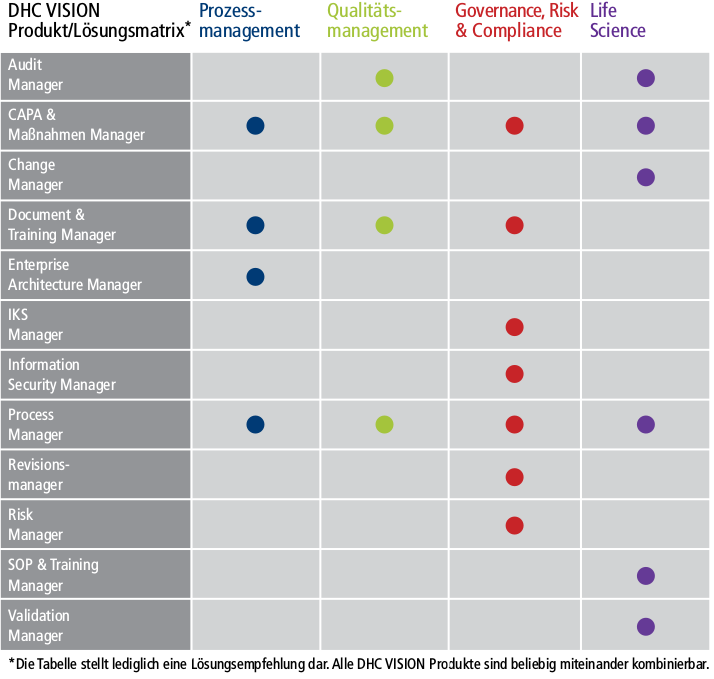
\includegraphics[scale=0.5]{images/dhc.png} 
\caption{DHC VISION Produkt/Lösungmatrix wie sie auf der Produktwebseite\cite{dhc} zu finden ist.}
\end{figure}

Die Features des Information Security Managers werden auf der Webseite\cite{dhc} wie folgt auszugsweise beschrieben:

\textbf{ISMS Management allgemein}
\begin{itemize}
\itemsep0em
\item IT-Strukturanalyse nach dem Standard des Bundesamts für Sicherheit in der Informationstechnologie (BSI) mit all ihren Komponenten und grafische Visualisierung
\item Schutzbedarfsfeststellung inkl. Beschreibung der Unternehmens-Assets mit Bedrohungen, Schwachstellen und Risiken, z.B. auch auf Basis von Katalogen, wie den BSI-Bausteinen
\item BSI-bestätigte Software zur Vorgehensweise gemäß IT-Grundschutz
\end{itemize}

\textbf{ISMS Maßnahmen-Management}
\begin{itemize}
\itemsep0em
\item Definition, Durchführung, Dokumentation und Nachverfolgung von Maßnahmen
\item Erinnerung an Termine bzgl. eingeleiteter Maßnahmen inkl. Eskalationsmechanismen
\item Prüfung der Wirksamkeit der eingeleiteten Maßnahmen
\item Konfigurierbare Workflows zur Abarbeitung und zum formalen Abschluss (inkl. elektronischer Signaturen) der Maßnahmen
\end{itemize}

\textbf{ISMS Dokumentation}
\begin{itemize}
\itemsep0em
\item Erstellung von Sicherheitskonzepten und anderen Dokumenten auf Basis hinterlegter evtl. auch gruppenspezifischer Vorlagen
\item Integration in die Geschäftsprozesse
\item Erfassung von Sicherheitsvorfällen zu Assets
\item Verlinkung zwischen den Dokumenten und zu anderen Objekten (wie Produkten) zur besseren Auffindbarkeit
\end{itemize}

\textbf{Weitere Funktionen}
\begin{itemize}
\itemsep0em
\item Übersichtliche System-Cockpits und rollenspezifische Zugänge
\item Intelligentes Mandantenkonzept für internationale Unternehmen (mehrere Standorte,  verschiedene Sprachen)
\item Nutzer-Akzeptanz durch Integration der Microsoft-Produkte (Visio, Word, Excel, Project)
\item Umfangreiches Berichtswesen sowie Reporting
\item Granulares Berechtigungs- und Zugriffskonzept auf alle Informationen
\end{itemize}

Es wurde angeboten einen Testserver aufzusetzen, dies hätte jedoch zu lange gedauert und ein zweitägiges Seminar zur Einführung erfordert. Ein Webinar zur Demonstration der Software wurde organisiert. Dieses kam allerdings aufgrund von Terminunstimmigkeiten nicht zustande. Daher konnte das Tool nicht bewertet werden. Da der Support sehr zuvorkommend ist und die angegebenen Features gut zu unseren Kriterien passen, wird eine weitere Beschäftigung mit dem Tool empfohlen.